%!TEX root = handout.tex

\section{Session 2 - The target-decoy approach}
In this part of the tutorial session two exercises regarding the manual computation of the target-decoy approach (TDA) will be conducted. Nowadays these tasks are performed automatically and "behind the scenes" by proteomics software tools and workflow engines. However, it is recommended to apply the TDA for some search engine results manually in order to get a better insight into the crucial FDR estimation for PSM identification.
\begin{figure}[ht]
	\centering
		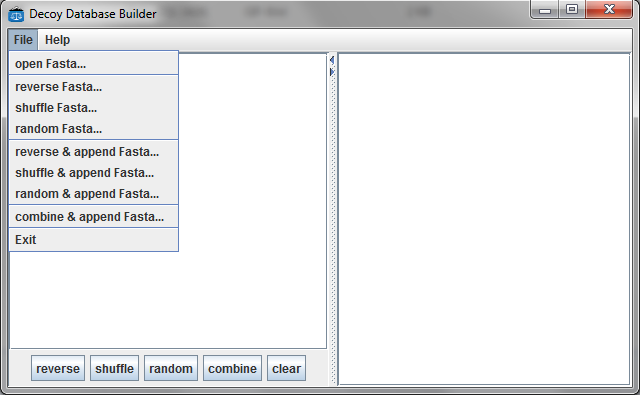
\includegraphics[scale=0.9]{graphics/targetdecoy/decoydatabasebuilder.png}
	\label{fig:decoydatabasebuilder}
	\caption{Screenshot of the tool \texttt{DecoyDatabaseBuilder}}
\end{figure}



\subsection{Exercise 1: Generate decoy databases}
Nowadays, the construction of decoy databases (decoy DBs) as well as the whole TDA and FDR estimation are hidden features of large proteomics software. Nevertheless, specific software tools are recommended and still in use in many labs in order to construct decoy DBs alternatively (in a way not supported by the large software used in the lab) or to perform a custom FDR estimation (e.g. different equations or different strategies for decoy generation). The \texttt{DecoyDatabaseBuilder} provided by the MPC is such a specific software for decoy DB construction. The java tool can be download from \menu{http://www.ruhr-uni-bochum.de/mpc/software/DecoyBuilder/index.html}. For this tutorial, the DecoyDatabaseBuilder can be found on the USB key.

\begin{task}
In order to construct decoy DBs please start the DecoyDatabaseBuilder by clicking on \texttt{DecoyDatabaseBuilder.jar}. Then, process the following DBs that are needed for the TDA-related workflows coming with this tutorial:
\begin{itemize}
	\item \directory{isb18mix.fasta}: by clicking \menu{reverse \& append Fasta...} and choosing this DB file (i.e., FASTA-file) please create a target-decoy DB by concatenation of the original DB and the DB of its reversed sequences.
	\item \directory{isb18mix.fasta} (again): by clicking \menu{shuffle \& append Fasta...} and choosing this DB file (i.e., FASTA-file) please create a target-decoy DB by concatenation of the original DB and the DB of its shuffled sequences.
	\item \directory{isb18\_plus\_yeast\_mod.fasta}: by clicking \menu{reverse \& append Fasta...} and choosing this DB file (i.e., FASTA-file) please create a target-decoy DB by concatenation of the original DB and the DB of its reversed sequences.
\end{itemize}
You will find the original FASTA-files on the flash drive (subfolder \newline{}\directory{databases\_and\_spectra} in the folder for this session). Please check the results that will be automatically saved in the source file folder by opening and inspecting them in a text editor (the basic notepad will not work, you can use e.g. Notepad++ or Vim)!
\end{task}



\subsection{Exercise 2: Load and run a KNIME-workflow for testing FDR formulas}
\textbf{Execute KNIME-workflow:} Switch to the workflow "GCB2015 I-3". Please correct your input and output paths for the nodes \KNIMENODE{Input File} (paths to the FASTA-file and the mzXML-file that can be found in the subfolder \directory{databases\_and\_spectra}) and \KNIMENODE{Output File} (e.g., the output folder \directory{exercise2} on the flash drive). Then, please run the workflow and check the two resulting csv files.

\begin{figure}
	\centering
		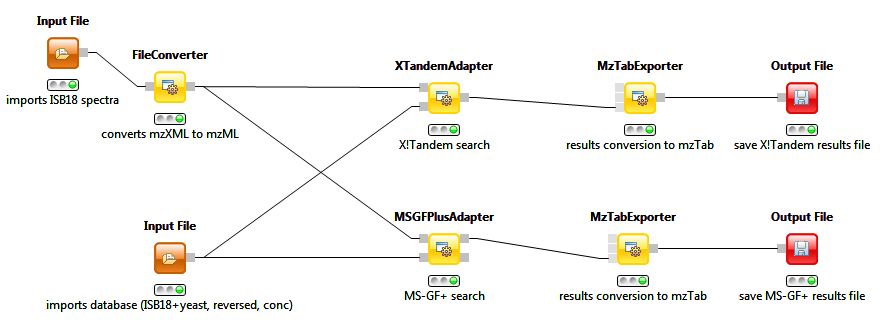
\includegraphics[scale=0.7]{graphics/targetdecoy/workflow_tda_i3.png}
	\label{fig:workflow_tda_i3}
	\caption{KNIME-workflow for exercise 2}
\end{figure}

\begin{task}

\texttt{Compute FDRs for X!Tandem results:} Now load the spectrum identification results csv file of the search engine "X!Tandem" (KNIME node: "XTandemAdapter") as well as the TDA template file "tda\_I3.xlsx" in Excel. Sort the data by means of the search engine score (here: from large to small values). In the highlighted columns of the template file the FDR estimation via TDA is performed. So, please apply the respective formulas given in the template to the X!Tandem results file.

\texttt{Compute FDRs for MS-GF+ results:} Now load the spectrum identification results csv file of the search engine "MS-GF+" (KNIME node: "MSGFPlusAdapter") as well as the TDA template file "tda\_I3.xlsx" in Excel. Sort the data by means of the search engine score (here: from small to large values). In the highlighted columns of the template file the FDR estimation via TDA is performed. So, please apply the respective formulas given in the template to the MS-GF+ results file.

\texttt{Explanation of the TDA-related columns in the template file:} In the following the columns of the TDA template file are explained:
\begin{itemize}
	\item \texttt{isDecoy:} For each position in the sorted data the current protein accession is checked whether it contains a specific tag indicating decoys proteins (e.g., in the example files "e" for reverse or "s" for shuffle). These tags are attached to decoy accessions by tools constructing decoy DBs.
	\item \texttt{decoyCount:} For each position of the sorted data the current number of decoys (i.e., $N_{decoys}$).
	\item \texttt{PSMcount:} For each position of the sorted data the current number of peptide spectrum matches (PSMs - i.e., $N_{psms} = N_{decoys}+N_{targets}$).
	\item \texttt{empFDR1:} Empirical FDR estimated via the formula
		\[ FDR_{empirical} = \frac{N_{decoys}}{N_{targets}} = \frac{N_{decoys}}{N_{psms}-N_{decoys}} \].
	\item \texttt{empFDR2:} Empirical FDR estimated via the alternative formula
		\[ FDR_{empirical} = \frac{2 \cdot N_{decoys}}{N_{targets}+N_{decoys}} \].
	\item \texttt{massError:} Computation of the relative parent mass error between the expected mass ($e$) and the calculated mass ($c$) for each peak in the spectrum in ppm via 
		\[ PME = \frac{e-c}{c \cdot 1,000,000} \].
	\item \texttt{isDummy:} Each PSM is checked whether it is a dummy PSM (i.e., whether the corresponding parent mass error $>$ 30 or whether the matched sequence is taken from the dummy yeast DB).
	\item \texttt{dummyCount:} For each position of the sorted data the current number of dummy PSMs (i.e., $N_{dummy}$).
	\item \texttt{factFDR:} The factual FDR estimated via the formula
		\[ FDR_{factual} = \frac{N_{dummy}+N_{decoys}}{N_{targets}} = \frac{N_{dummy}+N_{decoys}}{N_{psms}-N_{decoys}} \].
\end{itemize}

\texttt{Finally please complete this table as your final results:}

\end{task}

\begin{table}[htbp]
	\centering
		\begin{tabular}{|c|c|c|c|c|c|c|c|}
				Spectra & Database & ID tool & Formula & \multicolumn{2}{|c|}{empFDR at 5\%} & \multicolumn{2}{|c|}{factFDR fixed at 5\%}\\ \hline
				 &  &  &  & $N_{target}$ & factFDR & $N_{target}$ & empFDR\\ \hline\hline
				ISB18 & ISB18+yeast & X!Tandem & 1 &  &  &  & \\
				ISB18 & ISB18+yeast & MS-GF+ & 1 &  &  &  & \\
				ISB18 & ISB18+yeast & X!Tandem & 2 &  &  &  & \\
				ISB18 & ISB18+yeast & MS-GF+ & 2 &  &  &  & 
		\end{tabular}
	\caption{Exercise 2 results table}
	\label{tab:Exercise2Results}
\end{table}


\subsection{Additional exercise 3: Reversed decoy DB vs. shuffled decoy DB ("homework")}
\begin{task}
    \texttt{Execute KNIME-workflow:} Switch to the workflow "GCB2015 I-1" (reversing protein sequences as decoy construction approach). Please correct your input and output paths for the nodes \KNIMENODE{Input File} and \KNIMENODE{Output File} (see exercise 2). Then, please run the workflow and check the two resulting csv files. Please repeat this procedure for workflow "GCB2015 I-2" (shuffling as decoy construction approach). In total there will be four csv results files (for each decoy construction approach: one results file for the PSM identification tool "X!Tandem" and one for "MS-GF+").
    
    \texttt{Compute FDRs for X!Tandem results:} For each decoy construction approach calculate the FDR estimation in both csv results files (for X!Tandem and MS-GF+) following the formulas in the template file \directory{tda\_I1\_I2.xlsx}.
    
    \textbf{Compute FDRs for MS-GF+ results:} For each decoy construction approach calculate the FDR estimation in both csv results files (for X!Tandem and MS-GF+) following the formulas in the template file \directory{tda\_I1\_I2.xlsx}.
    
    \texttt{Explanation of the TDA-related columns in the template file:} see exercise 2 (only difference: dummy spectra are only defined by parent mass error threshold).

    \textbf{Finally please complete this table as your final results:}
\end{task}
\begin{table}[htbp]
	\centering
		\begin{tabular}{|c|c|c|c|c|c|c|c|}
				Spectra & Database & ID tool & decoyDB & \multicolumn{2}{|c|}{empFDR at 5\%} & \multicolumn{2}{|c|}{factFDR fixed at 5\%}\\ \hline
				 &  &  &  & $N_{target}$ & factFDR & $N_{target}$ & empFDR\\ \hline\hline
				ISB18 & ISB18+yeast & X!Tandem & reversed &  &  &  & \\
				ISB18 & ISB18+yeast & MS-GF+ & reversed &  &  &  & \\
				ISB18 & ISB18+yeast & X!Tandem & shuffled &  &  &  & \\
				ISB18 & ISB18+yeast & MS-GF+ & shuffled &  &  &  &
		\end{tabular}
	\caption{Exercise 3 results table}
	\label{tab:Exercise3Results}
\end{table}

